\documentclass[11pt]{article}

\usepackage{amsmath}
\usepackage{textcomp}
\usepackage[top=0.8in, bottom=0.8in, left=0.8in, right=0.8in]{geometry}
% Add other packages here %

%%Special equation notation sauce (not sure if I'll need it but it's nice not to have to think about it later)
\usepackage{amssymb}
\usepackage{mathtools}

%% declaring abs so that it works nicely
\DeclarePairedDelimiter\abs{\lvert}{\rvert}%
\DeclarePairedDelimiter\norm{\lVert}{\rVert}%

% Swap the definition of \abs* and \norm*, so that \abs
% and \norm resizes the size of the brackets, and the 
% starred version does not.
\makeatletter
\let\oldabs\abs
\def\abs{\@ifstar{\oldabs}{\oldabs*}}
%
\let\oldnorm\norm
\def\norm{\@ifstar{\oldnorm}{\oldnorm*}}
\makeatother



% Put your group number and names in the author field %
\title{\bf Exercise 1.\\ Implementing a first Application in RePast: A Rabbits Grass Simulation.}
\author{Group \textnumero: 272257, 262609}

\begin{document}
\maketitle

\section{Implementation}

%This section describes the main assumptions that were made in order to implement the simulation described on the Moodle.

\subsection{Assumptions}
% Describe the assumptions of your world model and implementation (e.g. is the grass amount bounded in each cell) %

\subsubsection{Assumptions for the Implementation of grass and of its growth}

There can be either $1$ or $0$ unit of grass per cell. At each simulation tick \textit{GrassGrowthRate} (default $50$) units of grass are added to empty cells \textbf{if possible}. This value is user defined and modifiable throughout the simulation.

\subsubsection{Assumptions for the Implementation of the movement of Rabbits and of collisions}

At each tick each alive rabbit tries to move to a random cell picked among the 4 cells adjacent to it's location. If it tries to move to a cell where another rabbit is present, \textbf{if the cell is empty it moves to it, if it is already occupied it doesn't move for this turn}. Regardless of whether it actually moved or not the rabbit loses $1$ energy unit per tick.

\subsubsection{Assumptions for the Implementation of feeding, energy and reproduction}

Each rabbit has an energy value $e \in [0,20]$. At each tick, if there exists a unit of grass on the cell it's on the rabbit "eats" it, it's energy increases by a user-set value. At each tick if a rabbit has an energy value $e \geq \text{ \textit{BirthThreshold}}$ it gives birth.

\subsubsection{Assumptions for the Implementation of birth and death}

When giving birth, \textbf{the parent rabbit gives a random proportion of it's energy to it's child}, meaning it losses some random amount of it's energy. The child inherits the exact amount of energy the parent lost when giving birth and appears on a random empty cell on the grid (the cell can have grass but no rabbit). The repartition of energy between parent and child is the following : $e_{parent} + e_{child} = e_{\text{\textit{parent before birth}}}$. At each tick, after movement, feeding, and reproduction rabbits whose energy is $\leq 0$, die: they are removed from the simulation.

\subsubsection{Assumptions for the initialization of the simulation}

The model is initialized with a user-set number of grass cells and rabbits. Initial rabbits are given a random amount of energy $e \in [0,20]$.

\subsection{Implementation Remarks}
% Provide important details about your implementation, such as handling of boundary conditions %

%The way the placement of new grass units and rabbits is handled is by picking a random position repeatedly until an empty cell is found, this operation can be repeated a finite number of times to avoid infinite loops in the case where no cell is free. This solution runs the risk of not finding a free spot in edge cases when there may actually be one but has the advantage of being relatively computationally inexpensive (in the most common case) compared to going through every single free cell every time. ==> commented out of the paragraph

In our model implementation energy is stored as a \textit{double} value. An alternative solution could be the storage of a separate list of every free cell but such an implementation would be quite memory-intensive for large size simulations.

\section{Results}
% In this section, you study and describe how different variables (e.g. birth threshold, grass growth rate etc.) or combinations of variables influence the results. Different experiments with different settings are described below with your observations and analysis

\begin{figure}[h!]
    \centering
    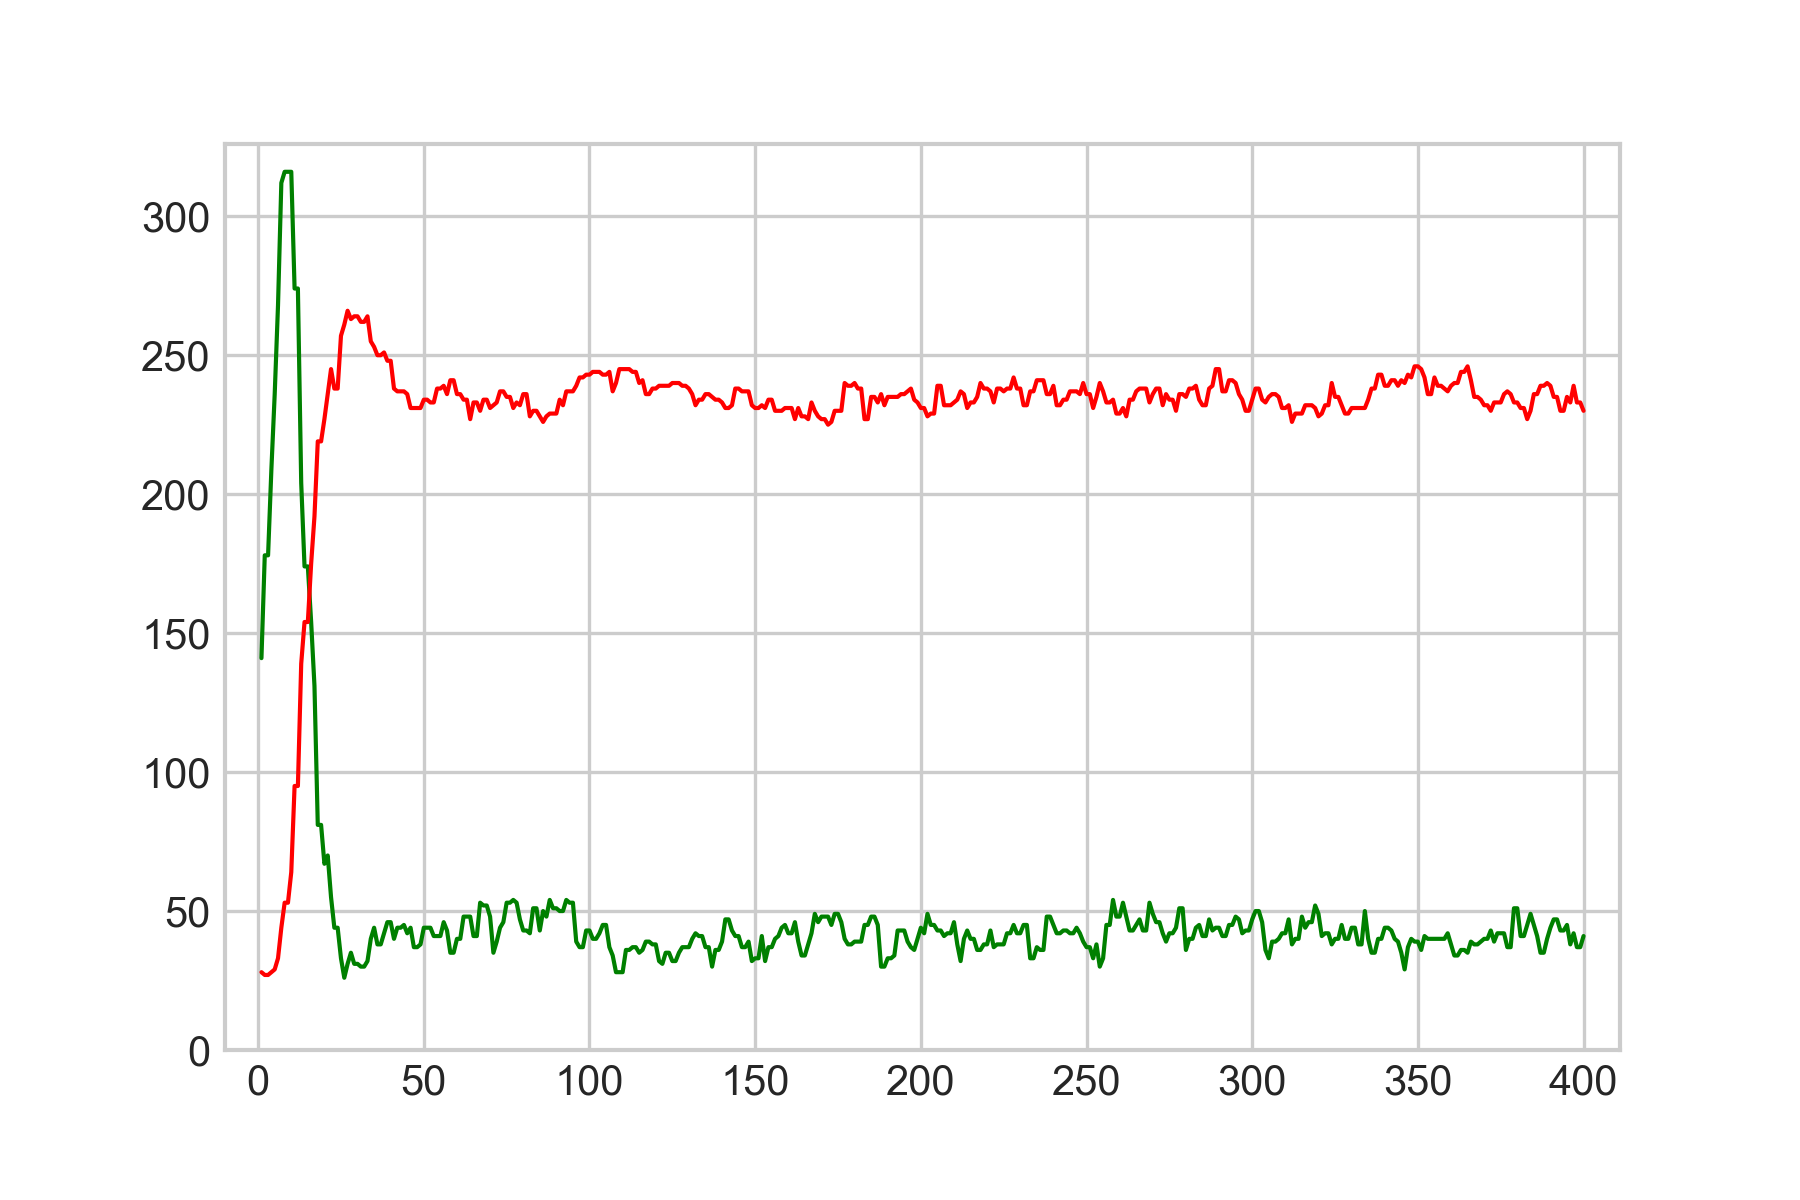
\includegraphics[width=0.4\textwidth]{plots/sim1.png}
    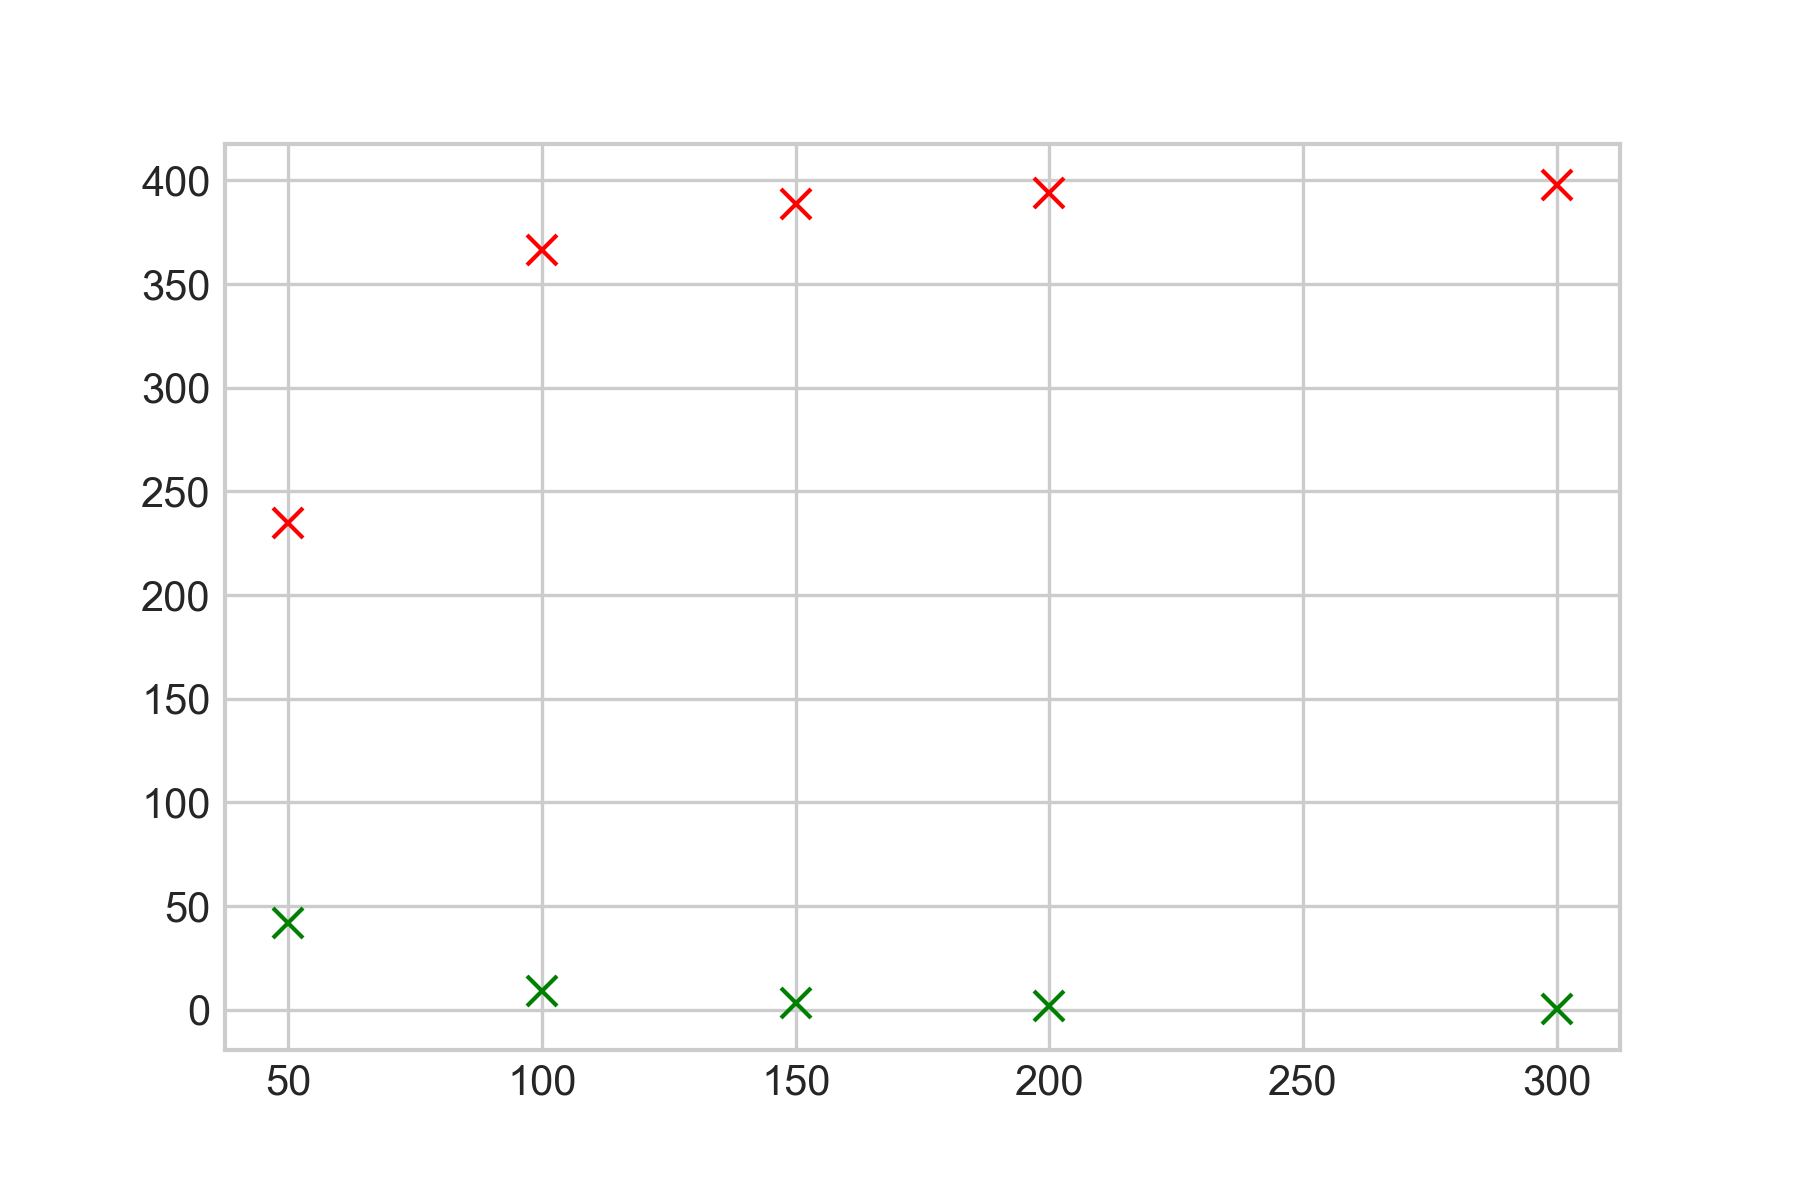
\includegraphics[width=0.4\textwidth]{plots/ggrate.png}
    \caption{\textbf{Right :} Lineplots of the rabbits (in red) and grass (in green) populations over the first 400 ticks of the reference simulation. \textbf{Left :} Evolution of rabbit (red) and grass (green) population equilibriums as the grass growth rate changes (each point pair here is a simulation).}
    \label{figure}
  \end{figure}

\subsection{Experiment 1 : reference run}

\subsubsection{Setting}

Default run : this will be our reference run. We will study the evaluation the simulation properties around those reference parameters.

\subsubsection{Observations} 

We observe that the default run (Figure \ref{figure}, left) converges in around $100$ ticks to a stable regime where the prey and predator populations (number of individuals) oscillate around equilibrium values. This is consistent with how typical solutions of Lokta-Volterra equations should behave.

% Elaborate on the observed results %

\subsection{Reaction of the simulation to variation in parameters}

We will now describe the way the model behaves in reaction to various parameters. First, let's observe that since the populations converge towards an equilibrium, as long as the initial populations of grass is sufficiently high so that the rabbit population does not die off, the initial populations values only have an influence on the transient response of the system, not on the stable state it converges to. \\

The grass growth rate is highly correlated with a high rabbit-to-grass population ratio, but saturates for high values see (Figure \ref{figure}, right). The grass energy behaves similarly (although it saturates for different reasons). The birth threshold of rabbits has an optimal value (around $15$) for a maximum rabbit-to-grass population ratio, this ratio gets lower for higher and lower values. \\

Finally a higher grid-size correlates to a higher grass-to-rabbit population ratio as well (and perhaps more interestingly) to a lower oscillation frequency in the stable mode.

\end{document}